\section*{1.7}
%\addcontentsline{toc}{section}{Question 1}

a) On sait que la vitesse d'une particule est en fait la dérivée de la position
par rapport au temps. On dénote la vitesse par $\dot{x}$, $x$ étant la position
de la particule. Nous avons alors l'équation différientielle suivante :
\begin{align*}
    \dot{x} = \dfrac{dx}{dt} &= e^{-t} + t\cos(t) + \sin(t),\ 
    x(0) = -1
\end{align*}

C'est une équation directement intégrable :
\begin{align*}
    \int{1\ dx} &= \int{(e^{-t} + t\cos(t) + \sin(t))\ dt} \\
    x(t) &= -e^{-t} + \int{t\cos(t)\ dt} -\cos(t) + C\\
    x(t) &= -e^{-t} + t\sin(t) + \cos(t) -\cos(t) + C\\
    x(t) &= -e^{-t} + t\sin(t) + C
\end{align*}

Avec la condition initiale donnée, on trouve que la solution particulière est :
\begin{align*}
    -1 &= -1 + 0 + C\\
    0 &= C \\
    \implies x(t) &= -e^{-t} + t\sin(t)
\end{align*}

b) À $t = 10$ et en faisant le calcul du sinus en radians,
la position de la particule est :
\begin{align*}
    x(10) &= -e^{-10} + 10\cdot\sin(10) \\
    x(10) &= -5.44
\end{align*}

Ensuite, à $t = 10$, la vitesse de la particule est :
\begin{align*}
    \dot{x}(10) &= e^{-10} + 10\cdot\cos(10) + \sin(10) \\
    \dot{x}(10) &= -8.93
\end{align*}

Finalement, pour trouver l'accélération, on dérive la vitesse de la particule
et on l'évalue à $t = 10$ :
\begin{align*}
    \ddot{x} &= -e^{-t} + \cos(t) - t\sin(t) + \cos(t)\\
    \ddot{x} &= -e^{-t} + 2\cos(t) - t\sin(t) \\
    \ddot{x}(10) &= -e^{-10} + 2\cos(10) - 10\cdot\sin(10) \\
    \ddot{x}(10) &= 3.76
\end{align*}

La particule se situe à 5.44 mètres à gauche de l'origine, elle se déplace à
une vitesse instantanée de 8.93 mètres par seconde vers la gauche et elle
décélère instantanément de 3.76 mètres par seconde par seconde.
\vspace{5mm}

c) Puisqu'il est difficile de déterminer de manière analytique et exacte le
nombre de fois que la particule passe par l'origine, on peut se fier au
graphique suivant. En particulier, on voit que la particule passe par l'origine
7 fois dans un laps de temps de 20 secondes :
\begin{center}
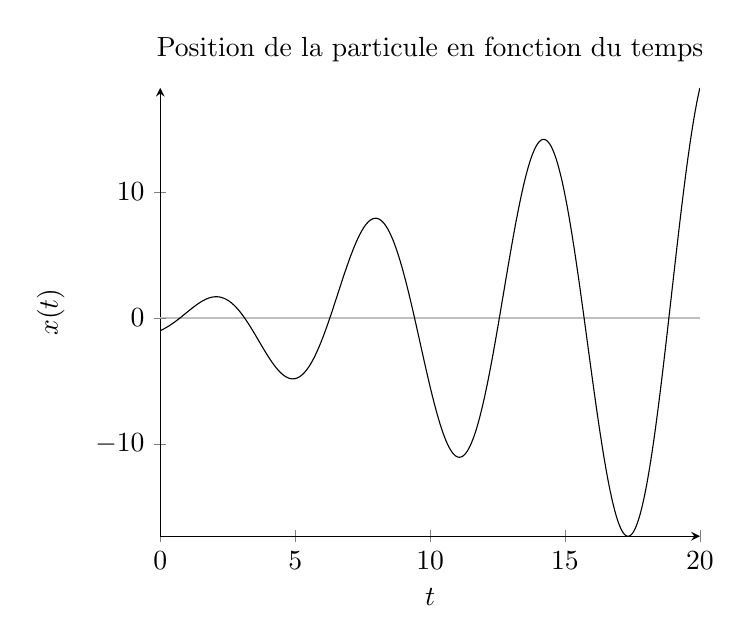
\begin{tikzpicture}
\begin{axis}[
    title = Position de la particule en fonction du temps,
    extra y ticks       = 0,
    extra y tick labels = ,
    extra y tick style  = { grid = major },
    axis lines = left,
    xlabel = \(t\),
    ylabel = {\(x(t)\)},
]
% Plot de la position
\addplot [
    domain=0:20, 
    samples=500, 
    color=black,
]
    {-1*e^(-1*x) + x*sin(deg(x))};
\end{axis}
\end{tikzpicture}
\end{center}
